% !TEX root = ../main.tex

\section{Implicit Differentiation}
Some curves' equations can't be solved for y (or maybe not easily), but we should still be able find the tangent line and its slope.
\begin{example}
    \begin{equation*}
        x^2 + y^2 = 4
    \end{equation*}
    \begin{itemize}
        \item Not a function!
        \item Can solve for $y$
    \end{itemize}
    \begin{equation*}
        y = \pm \sqrt{4 - x^2}
    \end{equation*}
    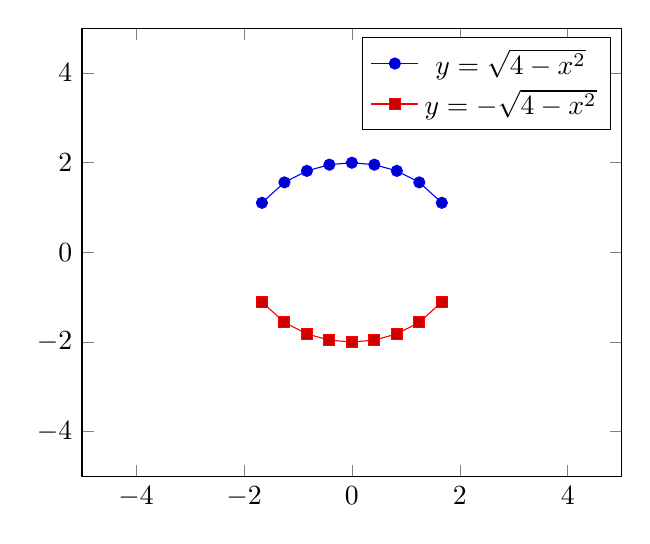
\begin{tikzpicture}
        \begin{axis}[xmin = -5, xmax=5, ymin=-5, ymax=5]
            \addplot +[blue]{sqrt(4 - x^2)};
            \addplot +[red]{-sqrt(4 - x^2)};
            \legend{$y = \sqrt{4 - x^2}$, $y = -\sqrt{4 - x^2}$};
        \end{axis}
    \end{tikzpicture}\\
    Given an expression with $x$s and $y$s to find $\deriv[y]$
    \begin{enumerate}
        \item Treat $y$ as a function of $x$ and differentiate both sides of the equation with respect to $x$
        \item Solve for $\deriv[y]$
        \item Win
    \end{enumerate}
    \begin{note}
        When doing step one (1), you can thing ``Whenever I thake the derivative of $y$ multiply that term by $\deriv[y]$.''
    \end{note}
    \begin{example}
        If $x^2 + y^2 = 4$ use implicit differentiation to find $\deriv[y]$
        
    \end{example}
\end{example}
